\documentclass{beamer}
\usetheme{default}
\usepackage{graphicx}
\usepackage{listings}
\usepackage{hyperref}

\title{Empaquetado en Debian}
\author{Emmanuel Arias}
\date{19 de octubre de 2024}
\begin{document}
\begin{frame}[plain]
    \maketitle
\end{frame}
\begin{frame}{Objetivo}
  \begin{itemize}
    \item Poder modificar un paquete existente.
    \item Crear nuestro propio paquete.
    \item Interactuar con la comunidad de Debian.
    \item Aprender lo mínimo para empaquetar, las cosas se aprenden con el día a día.
  \end{itemize}
\end{frame}

\begin{frame}
  \frametitle{¿Qué es Debian?}
	\begin{figure}
		\centering
		
\includegraphics[width=0.7\linewidth]{images/debian}
		\label{fig:debian}
	\end{figure}
\end{frame}

\begin{frame}
  \frametitle{¿Qué es Debian?}
	\begin{figure}
		\centering
		
\includegraphics[width=0.7\linewidth]{images/ian.jpg}
		\label{fig:debian}
	\end{figure}
\end{frame}

\begin{frame}
  \frametitle{Versiones de Debian}
	\begin{figure}
		\centering
		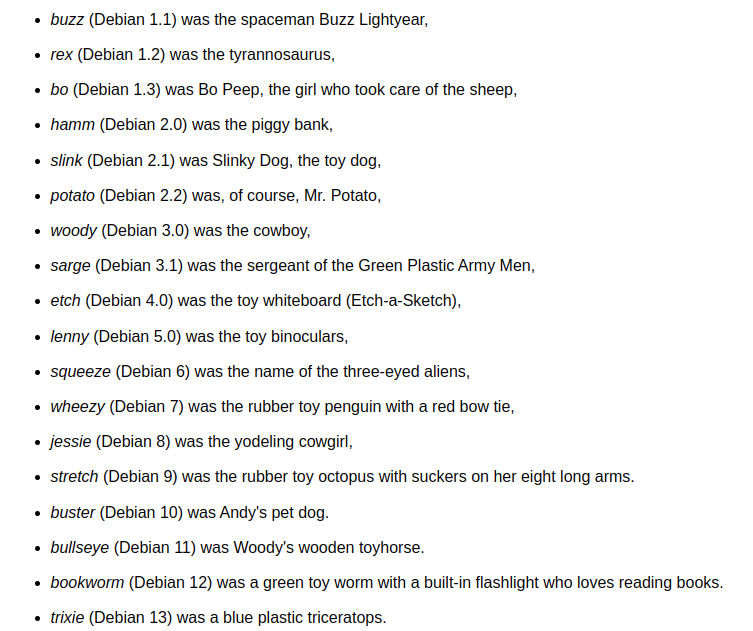
\includegraphics[width=0.7\linewidth]{images/versions.png}
		\label{fig:versiones de Debian}
	\end{figure}
\end{frame}
\begin{frame}
  \frametitle{Comunidad de Debian}
	\begin{figure}
		\centering
		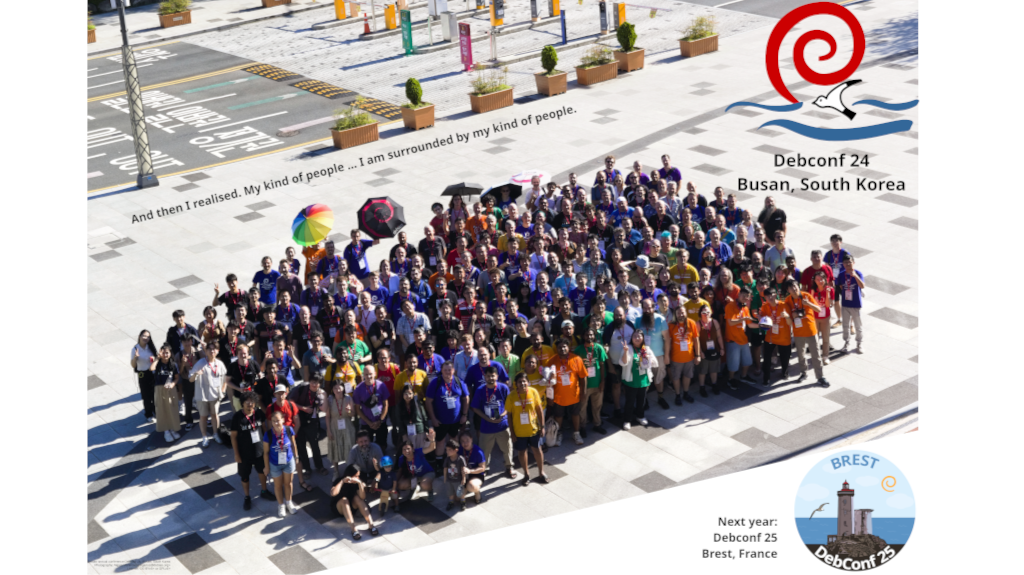
\includegraphics[width=0.7\linewidth]{images/debconf.png}
		\label{fig:comunidad de Debian}
	\end{figure}
\end{frame}

\begin{frame}{Debian}
  \begin{itemize}
    \item Tiene una cultura de excelencia ténica. Se crean releases cuando realmente estamos listos.
    \item Libertad. Desarrolladores y usuarios están beneficiados por el Contrato Social que promueve la cultura de Software Libre desde 1993.
    \item Independencia, no hay una empresa detrás de Debian.
  \end{itemize}
\end{frame}

\begin{frame}{Ciclo de releases}
 \begin{figure}
   \centering
   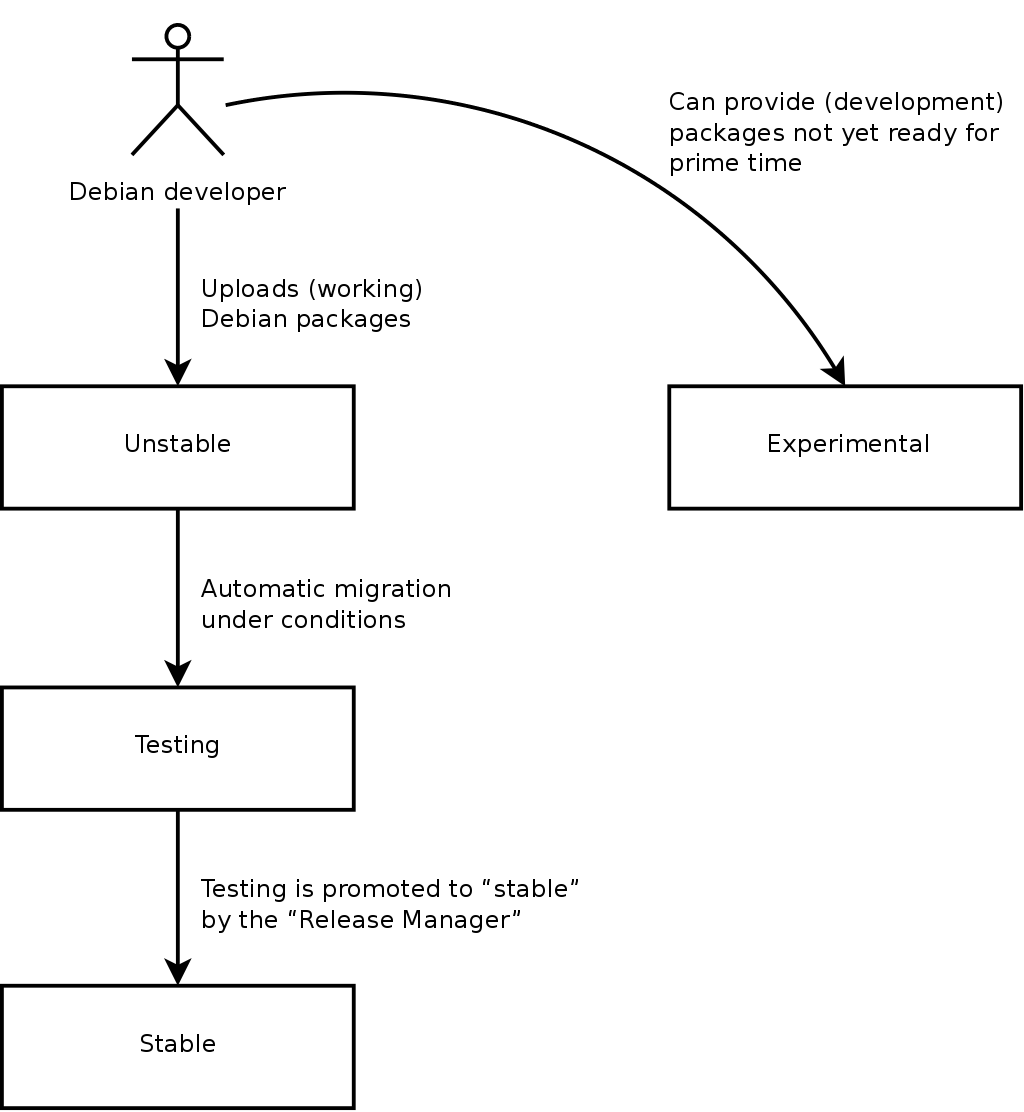
\includegraphics[width=0.7\linewidth]{images/release-cycle.png}
 \end{figure}
\end{frame}

\begin{frame}[fragile=singleslide]{Formato de los paquetes .deb}
  \begin{itemize}
  \item Los paquetes .deb son archivos ar
\begin{verbatim}
$ ar tv python3-mdit-py-plugins_0.4.1-1_all.deb
rw-r--r-- 0/0      4 May 16 22:52 2024 debian-binary
rw-r--r-- 0/0   2056 May 16 22:52 2024 control.tar.xz
rw-r--r-- 0/0  29348 May 16 22:52 2024 data.tar.xz
\end{verbatim}
  \item Podemos crear el paquete .deb con sus archivos manualmente: \url{https://tldp.org/HOWTO/html_single/Debian-Binary-Package-Building-HOWTO/}
  \end{itemize}
\end{frame}

\begin{frame}{Workflow}
 \begin{figure}
   \centering
   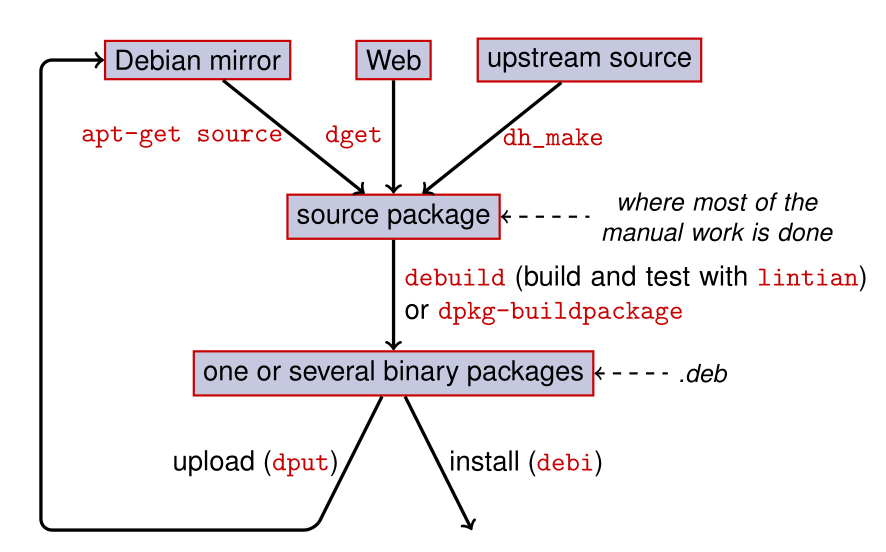
\includegraphics[width=0.7\linewidth]{images/workflow.png}
 \end{figure}
\end{frame}

\begin{frame}{Herramientas para instalar 0}
  \begin{itemize}
    \item build-essential (se asumen que está instalado en la máquina del desarrollador). Este incluye depndencia a dpkg-dev, que tiene las herramientas básicas para crear paquetes en Debian.
    \item devscripts
    \item git
    \item git-buildpackage
    \item sbuild
    \item sbuild-debian-developer-setup
    \item dh-make
    \item lintian
    \item autopkgtest
  \end{itemize}
\end{frame}


\begin{frame}{Herramientas para instalar 1}
  \begin{itemize}
    \item devscripts
    \item git
    \item git-buildpackage
    \item sbuild
    \item sbuild-debian-developer-setup
  \end{itemize}
\end{frame}

\begin{frame}[fragile=singleslide]{Setup del environment}
\begin{verbatim}
sudo apt install devscripts git git-buildpackage sbuild
sudo apt install sbuild-debian-developer-setup
 ...
sudo sbuild-debian-developer-setup
\end{verbatim}
\end{frame}

\end{document}
